On s'intéresse au développement d'une bactérie.

Dans cet exercice, on modélise son développement avec les hypothèses suivantes : cette bactérie a une probabilité $0,3$ de mourir sans descendance et une probabilité $0,7$ de se diviser en deux bactéries filles.

Dans le cadre de cette expérience, on admet que les lois de reproduction des bactéries sont les mêmes pour toutes les générations de bactéries qu'elles soient mère ou fille.

Pour tout entier naturel $n$, on appelle $p_n$ la probabilité d'obtenir au plus $n$ descendances pour une bactérie. 

On admet que, d'après ce modèle, la suite $\left(p_n\right)$ est définie de la façon suivante :

$p_0 = 0,3$ et, pour tout entier naturel $n$, \[p_{n+1} = 0,3 + 0,7p_n^2.\]
%

\begin{enumerate}
	\item La feuille de calcul ci-dessous donne des valeurs approchées de la suite $\left(p_n\right)$
	%
	\begin{center}
		\begin{tikzpicture}
			\tablineheight{6mm}
			\tableur*[19]{A/1.25cm,B/4cm}
			\celtxt*[c]{A}{1}{$n$}
			\celtxt*[c]{B}{1}{$p_n$}
			%1ère colonne
			\foreach \L in {2,3,...,19}{\celtxt*[c]{A}{\L}{\inteval{\L-2}}}
			%2ème colonne
			\celtxt*[c]{B}{2}{0,3}
			\celtxt*[c]{B}{5}{\num{0,40769562}}
			\celtxt*[c]{B}{6}{\num{0,416351}}
			\celtxt*[c]{B}{7}{\num{0,42134371}}
			\celtxt*[c]{B}{8}{\num{0,42427137}}
			\celtxt*[c]{B}{9}{\num{0,42600433}}
			\celtxt*[c]{B}{10}{\num{0,42703578}}
			\celtxt*[c]{B}{11}{\num{0,42765169}}
			\celtxt*[c]{B}{12}{\num{0,42802018}}
			\celtxt*[c]{B}{13}{\num{0,42824089}}
			\celtxt*[c]{B}{14}{\num{0,42837318}}
			\celtxt*[c]{B}{15}{\num{0,42845251}}
			\celtxt*[c]{B}{16}{\num{0,42850009}}
			\celtxt*[c]{B}{17}{\num{0,42852863}}
			\celtxt*[c]{B}{18}{\num{0,42854575}}
			\celtxt*[c]{B}{19}{\num{0,42855602}}
		\end{tikzpicture}
	\end{center}
	\begin{enumerate}
		\item Déterminer les valeurs exactes de $p_1$ et $p_2$ (masquées dans la feuille de calcul) et interpréter ces valeurs dans le contexte de l'énoncé.
		\item Quelle est la probabilité, arrondie à $10^{-3}$ près, d'obtenir au moins 11 générations de bactéries à partir d'une bactérie de ce type ?
		\item Formuler des conjectures sur les variations et la convergence de la suite $\left(p_n\right)$.
	\end{enumerate}
	\item 
	\begin{enumerate}
		\item Démontrer par récurrence sur $n$ que,
		pour tout entier naturel $n$, $0 \leqslant p_n \leqslant p_{n+1} \leqslant0,5$.
		\item Justifier que la suite $\left(p_n\right)$ est convergente.
	\end{enumerate}
	\item On appelle $L$ la limite de la suite $\left(p_n\right)$.
	\begin{enumerate}
		\item Justifier que $L$ est solution de l'équation \[0,7x^2 - x  + 0,3 = 0.\]
		\item Déterminer alors la limite de la suite $\left(p_n\right)$.
	\end{enumerate}
	\item La fonction suivante, écrite en langage \textsf{Python}, a pour objectif de renvoyer les $n$ premiers termes de la suite $\left(p_n\right)$.
	
\begin{CodePythonLstAlt}*[Largeur=8cm]{center}
def suite(n) :
	p = ...
	s = [p]
	for i in range(...) :
		p = ...
		s.append(p)
	return (s)
\end{CodePythonLstAlt}
	Recopier, sur votre copie, cette fonction en complétant les lignes 2, 4 et 5 de façon à ce que la fonction \texttt{suite(n)} retourne, sous forme de liste, les $n$ premiers termes de la suite.
\end{enumerate}